\documentclass[notitlepage, reprint, nofootinbib]{revtex4-1}
\usepackage[utf8]{inputenc}

% Mathematics and symbols:
\usepackage{amsmath, gensymb, amsthm, physics, mhchem}
% Figures:
\usepackage{tikz, graphicx}
\usepackage[caption=false]{subfig}

% Other:
\usepackage{hyperref}


% Document formatting 
\setlength{\parskip}{1mm}
\setlength{\parindent}{0mm}

% Programming
\definecolor{codebackground}{rgb}{0.9,0.9,0.9}
\usepackage{listings}
\lstset{
	language=python,
	backgroundcolor=\color{codebackground},
	basicstyle=\scriptsize,
	aboveskip={1\baselineskip},
	columns=fixed,
	numbers=left,
	showstringspaces=false, 
	breaklines=true, 
	frame=single,
	showtabs=false,
	showspaces=false,
	keywordstyle=\color[rgb]{0,0,1},
	commentstyle=\color[rgb]{0.133,0.545,0.133}
	}

%\renewcommand{\thesubsubsection}{\alph{subsubsection})}

\hypersetup{
    colorlinks=true,
    linkcolor=blue,
    filecolor=magenta,      
    urlcolor=cyan,
}

\begin{document}
\title{FYS3150 - Project 1}
\author{Frida Larsen}
\maketitle

% Introduction
\section{Introduction}
{\color{red}{Reference code in github repository.}}\\[2mm]
The one-dimensional Poisson equation is given by 
\begin{equation}\label{Poisson}-\dv[2]{x} u(x)=f(x),\end{equation}
with Dirichlet boundary conditions
\begin{equation}\label{Dirichlet}u(0)=u(1)=0\end{equation}
on the interval $x\in (0,1)$.

% Theory
\section{Theory}
The second derivative of a general discretized function $g_i$ can be approximated by 
\begin{equation}\label{second_derivative} g_i'' \approx \frac{g_{i+1}+g_{i-1}-2g_i}{h^2}\end{equation}
The discretized version of the Poisson equation (\ref{Poisson}) then becomes 
\begin{equation}\label{Poisson_discrete}-\frac{u_{i+1}+u_{i-1}-2u_i}{h^2}=f_i,\end{equation}
where we have defined the discretized approximation to $u$ and $x$ as $u_i$ and $x_i$ respectively, such that $x_i=ih$, $x_0=0$ and $x_{n+1}=1$. We also have $f_i=f(x_i)$. The step length $h$ is defined as 
\begin{equation}\label{step_length}h=\frac{1}{n+1},\end{equation}
where $n$ is the total number of grid points on the interval (0,1). The Dirichlet boundary conditions (\ref{Dirichlet}) become
\begin{equation}\label{Dirichlet2}u_0=u_{n+1}=0.\end{equation}
The discrete Poisson equation can be further simplified as
$$-u_{i+1}-u{i-1}+2u_i=h^2f_i.$$
By introducing $\tilde{b}_i=h^2f_i$ and remembering that $u_0=0$ the Poisson equation for the first few $i$-values are
\begin{align*}
	i=1:&\quad 2u_1-u_2=\tilde{b}_1\\
	i=2:&\quad -u_1+2u_2-u_3=\tilde{b}_2\\
	i=3:&\quad -u_2+2u_3-u_4=\tilde{b}_3\\
	&\dots
\end{align*}
This set of equations can be rewritten as a matrix equation 
\begin{equation}\label{lil_boi}\vb{A}\vb{u}=\vb{\tilde{b}}\end{equation}
with
\begin{equation}\label{big_boi}\vb{A}=\mqty( 2 & -1  & 0 &\dots &\dots &0\\-1&2&-1&0&\dots&\dots\\0&-1&2&-1&0&\dots\\ \dots&\dots&\dots&\dots&\dots&\dots \\ 0&\dots&\dots&-1&2&-1\\ 0&\dots&\dots&0&-1&2 ).\end{equation}


% Method
\section{Method}
{\color{red}{Include closed-form solution here as a part of unit test maybe??}}\\[2mm]
In order to develop an algorithm for solving the matrix equation (\ref{lil_boi}) we will begin with a general $n\times n$ tridiagonal matrix 
\begin{equation}\label{big_boi_bro}\vb{\tilde{A}} = \mqty(b_1&c_1&0&\dots&\dots&\dots\\a_1&b_2&c_2&0&\dots&\dots\\0&a_2&b_3&c_3&0&\dots\\ \dots&\dots&\dots&\dots&\dots&\dots\\ \dots&\dots&0&a_{n-2}&b_{n-1}&c_{n-1}\\ \dots&\dots&\dots&0&a_{n-1}&b_n)\end{equation}
{\color{red}{Reference Tridiagonal Matrix Algorithm}} on Wikipedia. \\[2mm]
\textbf{Algorithm 1:} The first step is a forward substitution, 
\begin{equation}c_i' =\begin{cases} \frac{c_i}{b_i}&; \quad i=1\\ \frac{c_i}{b_i-a_ic_{i-1}'}&;\quad i=2,3,\dots,n-1\end{cases}\end{equation}
and 
\begin{equation}\tilde{b}_i'=\begin{cases}\frac{\tilde{b}_i}{b_i}&;\quad i=1\\ \frac{\tilde{b}_i-a_i\tilde{b}_{i-1}'}{b_i-a_ic_{i-1}'}&;\quad i=2, 3,\dots,n\end{cases}\end{equation}
The second step is to obtain the solution by back substitution, 
\begin{align}
	u_n=\tilde{b}_n'&; \quad i=n\\
	u_i=\tilde{b}_i'-c_i'u_{i+1}&;\quad i=n-1,n-2,\dots,1.
\end{align}
\textbf{Algorithm 2:} Although the above algorithm works for the matrix belonging to our Poisson equation, the generalized $\vb{\tilde{A}}$ is actually more complicated than our original $\vb{A}$. A more accurate generalization would be 
\begin{equation}\label{another_big_boi}\vb{A}_g = \mqty(b_1&a_1&0&0&\dots&0\\a_2&b_2&a_2&0&\dots&0\\0&a_3&b_3&a_3&\dots&0\\ 0&\dots&\dots&\dots&\dots&\dots\\ \dots&\dots&\dots&\dots&\dots&a_{n-1}\\ \dots&\dots&\dots&\dots&a_n&b_n),\end{equation}
where the upper and lower diagonals consist of the same elements. We observe that 
$$\vb{A}\ \ \mqty{\uppercase\expandafter{\romannumeral 2}-\frac{a_2}{b_2}\uppercase\expandafter{\romannumeral 1}\\ \sim}\ \mqty(b_1&a_1&0&0&\dots&0\\0&\tilde{b}_2&a_2&0&\dots&0\\0&a_3&b_3&a_3&\dots&0\\ 0&\dots&\dots&\dots&\dots&\dots\\ \dots&\dots&\dots&\dots&\dots&a_{n-1}\\ \dots&\dots&\dots&\dots&a_n&b_n),$$
with $\tilde{b}_2=b_2-\frac{a_2a_1}{b_1}$. Repeating this process for all rows 1 to $n$ results in the lower diagonal being replaced by 0's only and the diagonal b's being replaced by 
\begin{equation}\label{b_tilde_ein} \tilde{b}_i=\begin{cases} b_1, \quad &i=1 \\ b_i - \frac{a_i a_{i-1}}{\tilde{b}_{i-1}},\quad &i=2, 3,\dots, n\end{cases}\end{equation}
Applying this process to the right hand side of equation \ref{lil_boi} we get
\begin{equation}\label{f_tilde_ein}\tilde{f}_i=\begin{cases}f_1,\quad &i=1\\ f_i-\frac{a_i \tilde{f}_{i-1}}{\tilde{b}_{i-1}},\quad&i=2,3,\dots,n\end{cases}\end{equation}
Substituting these expressions backwards into the matrix equation {\ref{lil_boi}} we find the solution
\begin{equation}\label{general_u_ein}u_i=\begin{cases}\frac{\tilde{f}_i}{\tilde{b}_i},\quad&i=n\\ \frac{\tilde{f}_i-a_i u_{i+1}}{\tilde{b}_i},\quad&i=n-1,n-2,\dots,1\end{cases}\end{equation}
Although these expressions are much simpler than those for algorithm 1, there are further simplifications to be made. For our original matrix (\ref{big_boi}) all the $a$'s are -1 and all the $b$'s are 2. Inserting this yields
\begin{align}
	\tilde{b}_i &= \begin{cases}2,\quad&i=1\\2-\frac{1}{\tilde{b}_{i-1}},\quad&i=1,2,\dots,n\end{cases}\nonumber\\
	&=\frac{i+1}{i},\quad \quad \quad \ \ \ i=1,2,\dots, n,\label{algo2b}
\end{align}
which leads to
\begin{align}
	\tilde{f}_i&=\begin{cases}f_1,\quad &i=1\\f_i+\frac{\tilde{f}_{i-1}}{i/(i-1)},\quad&i=2,3,\dots, n\end{cases}\nonumber\\
	&=f_i+\frac{(i-1)\tilde{f}_{i-1}}{i},\quad i=1,2,\dots,n\label{algo2f}
\end{align}
and finally 
\begin{equation}\label{algo2u}u_{i-1}=\frac{i-1}{i}(\tilde{f}_{i-1}+u_i),\ i=n,\dots,2\end{equation}
with $u_n=\tilde{f}_n/\tilde{b}_n$.\\[2mm]
In order to test these algorithms, we will use a function for the right hand side of the matrix equation (\ref{lil_boi}) given by
\begin{equation}\label{test_func}\tilde{b}(x)= h^2 100e^{-10x},\end{equation}
with closed-form solution 
\begin{equation}\label{test_func_sol}u_s(x)=1-(1-e^{-10})x-e^{-10x}.\end{equation}



% Results
\section{Results}
Figure \ref{fig1} shows plots of the algorithm solution as compared to the closed-form solution of the matrix equation (\ref{lil_boi}) with the general $\vb{\tilde{A}}$ as given by equation \ref{big_boi_bro} for three different sized matrices. We see that the curves with more grid points are closer to the closed-form solution. 

\begin{figure}
	\centering
	\subfloat[Comparison using n=10 grid points.]{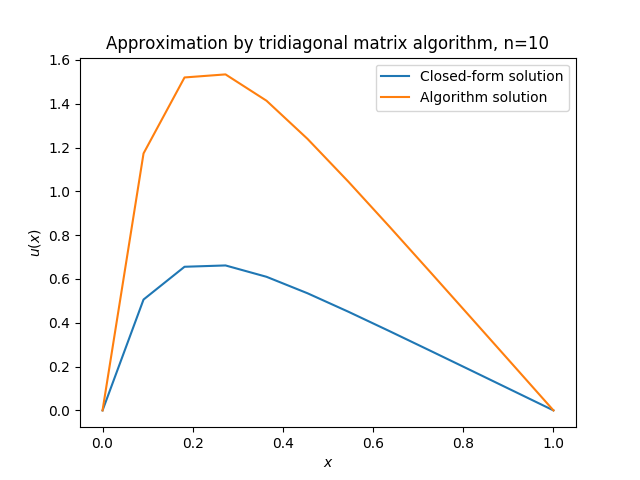
\includegraphics[width=0.5\textwidth]{../Figures/t_m_a_n_10.png}}
	\hfill
	\subfloat[Comparison using n=100 grid points.]{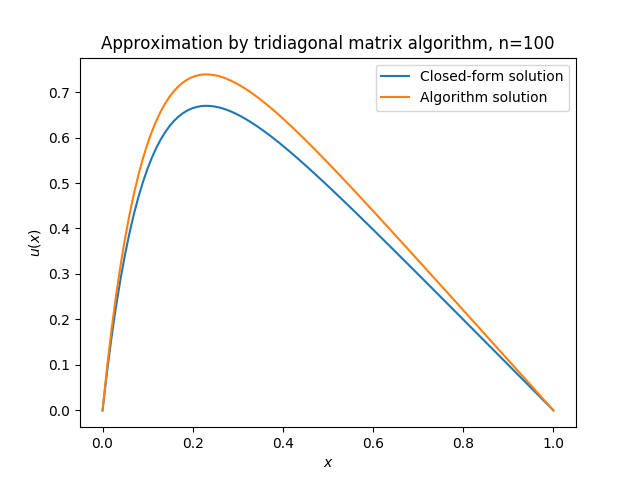
\includegraphics[width=0.5\textwidth]{../Figures/t_m_a_n_100.png}}
	\hfill
	\subfloat[Comparison using n=1000 grid points.]{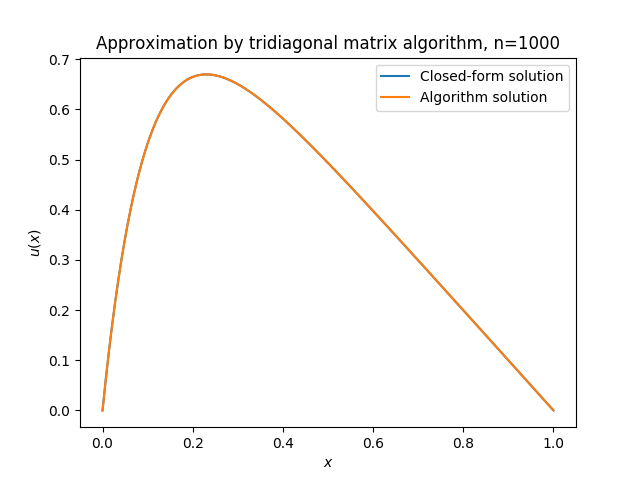
\includegraphics[width=0.5\textwidth]{../Figures/t_m_a_n_1000.png}}
	\caption{Comparison of the tridiagonal matrix algorithm and the analytical solution for the function $\tilde{b}$ (\ref{test_func}) for different sized matrices.}
	\label{fig1}
\end{figure}

% Discussion
\section{Discussion}

% Conclusion
\section{Conclusion}
















\end{document}